\documentclass[12pt]{article}
\usepackage{amsmath}
\usepackage{amssymb}
\usepackage{geometry}
\usepackage{enumerate}
\usepackage{natbib}
\usepackage{float}%稳定图片位置
\usepackage{graphicx}%画图
\usepackage[english]{babel}
\usepackage{a4wide}
\usepackage{indentfirst}%缩进
\usepackage{enumerate}%加序号
\usepackage{multirow}%合并行
\title{\large UM-SJTU JOINT INSTITUTE\\Major Design Experience\\(VE450)\\\ \\\
\begin{figure}[H]
\centering
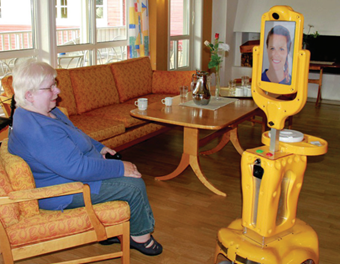
\includegraphics[scale=0.5]{P1.png}
\end{figure}
Design Review Report\\\  Telepresence Robot for Elderly \\\ \\\ \\\ Sponsor: JI CFE as part of mHBR initiative \\\ Mentor: Prof. Pradeep Ray, Prof. Artur Serrano \\\ Instructor: Prof. Guo Yunlong }
\author{Pan Chongdan\qquad  panddddda@sjtu.edu.cn\\Boaro Fernando\\Liu Niyiqiu\\Qiu Tianyu\\Zhou Ruixing}
\date{Date: \today}
\begin{document}
\maketitle
\newpage
\section{Abstract}
\subsection{Project Motivation and Outcomes}
The telepresence robot for elderly mainly aims at providing remote care for the elderly when their caregivers are far away from them. Indeed, the robot can play a row as an alternative of personal visits and provide a real network of care. 
\par Nowadays, there are telepresence robots products used in Europe now, and relative research shows they indeed increased feelings of happiness, self-esteem and reduced levels of frustration of their users.However, they're extremely expensive and hard to operate because a lot of limitations like unstable network communication caused by firewall. Therefore, we want to simplify and stabilize the robot so that the robot can be used by more people.
\par As far as our primary initial design, we want to realize stable remote control, visual communication and medicine dispensers. With such functions, the telepresence can maximize its value and provide a emotional belt between the elderly and caregivers. 
\subsection{Specification}
A general image of our robot will be a tall screen based on a self-moving chassis. The core processor will be connect to the Internet so that the caregivers can control it. The height of the robot will be about 1m so that it's easy for the elderly to operate. The length and width of the robot is within 0.6m so that it can move with flexibility indoors. For safety, the robot won't operate at voltage higher than 20V and there are less than 10 motors on the robot. The screen will be about 7 inch on diagonal with touch function.
\subsection{Main Problem and Challenge} 
\par The project including following design problems:
\begin{enumerate}[-]
\item Design, build and test the robot under the cost of 1000 dollars.
\item Providing stable and instant communication with the elderly and caregivers even when they're very far away from each other. 
\item Establish a system so stable that the caregivers can control the movement of the robot easily with help from vision sensors.
\item Build medicine dispenser to distribute pills to the elderly.
\end{enumerate}
\subsection{Project Plan}
We want to make our first prototype in October, then Pan Chongdan will communicate with our sponsors at Norway and get some feedbacks. In November, we'll do some improvement and try to stabilize the robot.
\section{Introduction \& Problem Description }
With the acceleration of life rhythm, people usually spends more time away from home, causing more loneliness for the elderly. Under the circumstances, caregivers will be worried about the elderly's well-being and the elderly may feel a loss of bond with family and children. Telepresence robot is designed to cope with such scenario because caregivers can communicate and provide care for the elderly with the robot when they're away. From emotion perspective, the telepresence can play a role as an substitute of the caregivers so that it can enhance the connection between the elderly and their children
\subsection{Problem}
\begin{enumerate}[1]
\item \textbf{Budget}
\par Our budget is under 1000 dollars while the products in the market is much more expensive than that, which implies that it will take much money to relative the robot's functions. The biggest problem for us is to redesign, simplify the robot and realize the essential functions without spending a lot of money.
\item \textbf{Telepresence Technology}
\par The core technology of telepresence robot is to establish stable and simple connection between the controller and the robot. Since firewall and routers are often used, there are many obstacles impeding the transmission of control signal. What's more, since the caregivers will keep moving, so the mobility of such control system is very important.
\item \textbf{Stable Control System} 
\par To realize available control between the caregivers and the robot, core processor, actors and sensors are essential. First we need to control actuators by giving instructions to the core processor connected the network. Then feedbacks will be given by sensors so that the caregivers can know the status of the robot. One of the most important task for our team is to create a available interface between the robot and caregivers so that they can control it smoothly.
\item \textbf{Functions for the elderly}
\par It's important to realize functions specially for the elderly. Since the elderly usually have different needs and different characteristics, the robot should be able to cope with different kinds of people. For example. different old people have different pills to eat at different time, so the medicine dispenser should be flexible enough to coordinate with it. It should be able to dispense various pills at once.
\item \textbf{Safety and Power}
\par Since usually the elderly usually stay with the robot alone, safety is very important and the nominal voltage shouldn't be too high, which is less than 30V. In addition, the robot should has a battery of high capacity so that it doesn't need frequent charging because it's hard for the elderly to bow and deal with the power supply.
\end{enumerate}
\subsection{Competitive and Related Products or Technology}
\subsubsection{Giraffe Telepresence Robot}
All the similar products in market right now is much more expensive than 1000 dollars, and the most representative product is \textbf{Giraffe} produced by a Europe company.
\begin{figure}[H]
\centering
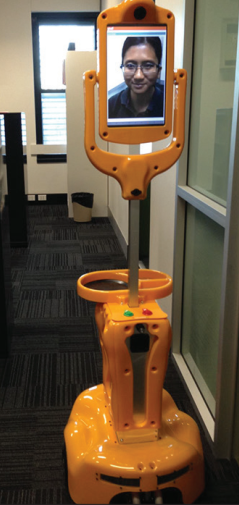
\includegraphics[scale=1]{P2.png}
\end{figure}
Giraffe has been put into the market for some time and it does have an effect on providing care and emotional connection to the elderly. However, it still have some problems such as firewall issues, video freezing, and driving lag etc, but it can be a reference based on which we can design and build our own telepresence robot.
\par In China, there is no such robot products but some smart furniture can be our competitive products
\subsubsection{Raspberry Pi}
\begin{figure}[H]
\centering
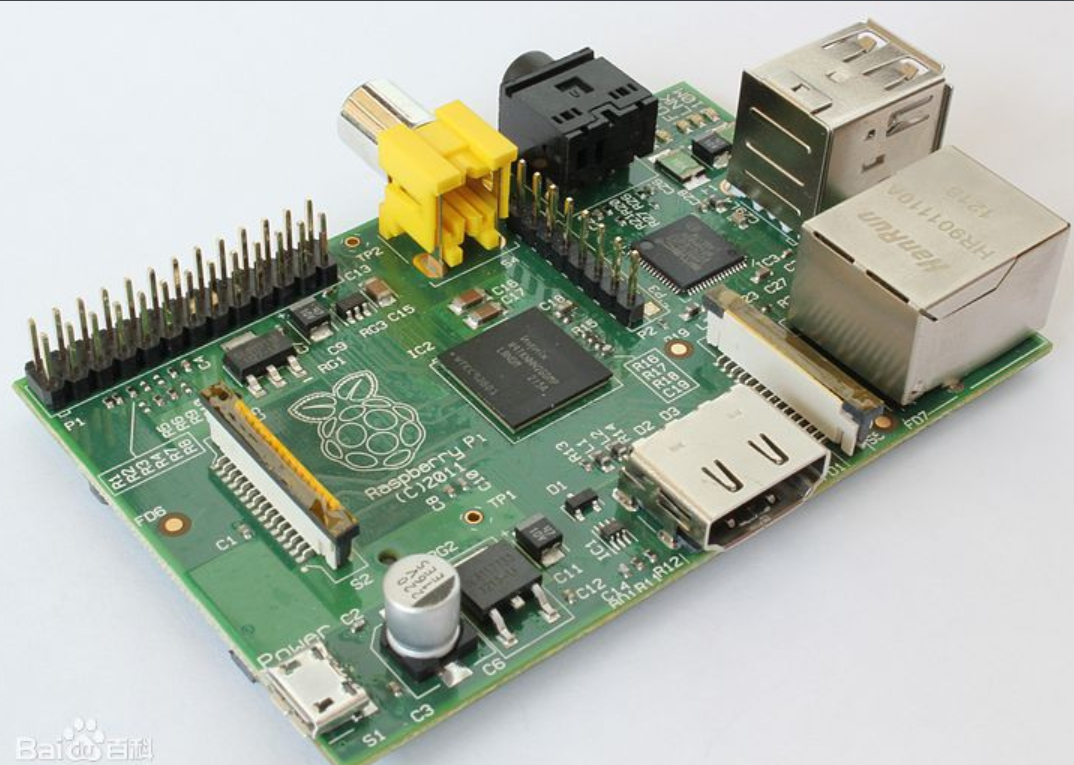
\includegraphics[scale=0.15]{P3.png}
\end{figure}
Raspberry Pi is a micro computer with many I/O interface so that it's easy for us to develop and control functions based on it. In addition. sin raspberry has its own linux system, we can write some control codes and realize Internet connection through it. Raspberry Pi can be a good central core for the telepresence robot.
\subsubsection{Team Viewer}
\begin{figure}[H]
\centering
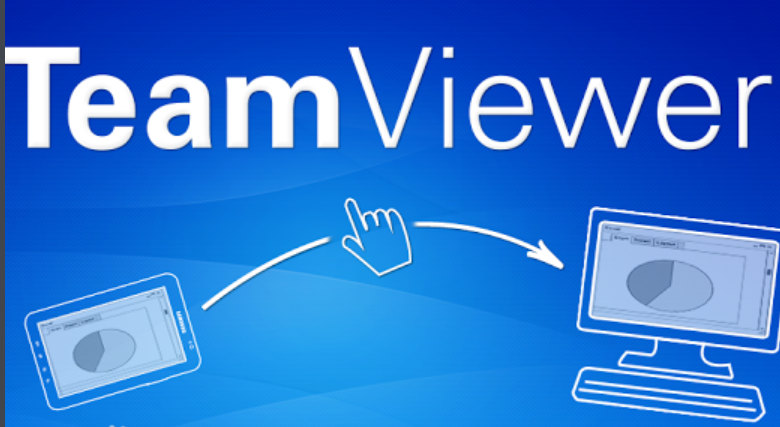
\includegraphics[scale=0.3]{P4.png}
\end{figure}
Team Viewer is a software developed by Germany which can provide stable remote control between different computers. What's more team viewer can be applied on any devices connected to world wide web as long as it has its own operating system. Team viewer is an important technology to realize stable remote control and control mobility of telepresence
\subsection{Screen, Camera and other Actuators and Sensors}
There is big screen which can be connected to the raspberry pi. With such screen, the elderly can communicate with the caregivers visually and freely. On the other hand, camera like opencv can get pictures from the elderly or the surrounding environment for the caregivers so that they can control the robot and contact the elderly more easily. Actuators and sensors will play an auxiliary role for realize such functions.
   
\end{document}